% Options for packages loaded elsewhere
\PassOptionsToPackage{unicode}{hyperref}
\PassOptionsToPackage{hyphens}{url}
\PassOptionsToPackage{dvipsnames,svgnames,x11names}{xcolor}
%
\documentclass[
  letterpaper,
  DIV=11,
  numbers=noendperiod]{scrartcl}

\usepackage{amsmath,amssymb}
\usepackage{iftex}
\ifPDFTeX
  \usepackage[T1]{fontenc}
  \usepackage[utf8]{inputenc}
  \usepackage{textcomp} % provide euro and other symbols
\else % if luatex or xetex
  \usepackage{unicode-math}
  \defaultfontfeatures{Scale=MatchLowercase}
  \defaultfontfeatures[\rmfamily]{Ligatures=TeX,Scale=1}
\fi
\usepackage{lmodern}
\ifPDFTeX\else  
    % xetex/luatex font selection
\fi
% Use upquote if available, for straight quotes in verbatim environments
\IfFileExists{upquote.sty}{\usepackage{upquote}}{}
\IfFileExists{microtype.sty}{% use microtype if available
  \usepackage[]{microtype}
  \UseMicrotypeSet[protrusion]{basicmath} % disable protrusion for tt fonts
}{}
\makeatletter
\@ifundefined{KOMAClassName}{% if non-KOMA class
  \IfFileExists{parskip.sty}{%
    \usepackage{parskip}
  }{% else
    \setlength{\parindent}{0pt}
    \setlength{\parskip}{6pt plus 2pt minus 1pt}}
}{% if KOMA class
  \KOMAoptions{parskip=half}}
\makeatother
\usepackage{xcolor}
\setlength{\emergencystretch}{3em} % prevent overfull lines
\setcounter{secnumdepth}{-\maxdimen} % remove section numbering
% Make \paragraph and \subparagraph free-standing
\ifx\paragraph\undefined\else
  \let\oldparagraph\paragraph
  \renewcommand{\paragraph}[1]{\oldparagraph{#1}\mbox{}}
\fi
\ifx\subparagraph\undefined\else
  \let\oldsubparagraph\subparagraph
  \renewcommand{\subparagraph}[1]{\oldsubparagraph{#1}\mbox{}}
\fi

\usepackage{color}
\usepackage{fancyvrb}
\newcommand{\VerbBar}{|}
\newcommand{\VERB}{\Verb[commandchars=\\\{\}]}
\DefineVerbatimEnvironment{Highlighting}{Verbatim}{commandchars=\\\{\}}
% Add ',fontsize=\small' for more characters per line
\usepackage{framed}
\definecolor{shadecolor}{RGB}{241,243,245}
\newenvironment{Shaded}{\begin{snugshade}}{\end{snugshade}}
\newcommand{\AlertTok}[1]{\textcolor[rgb]{0.68,0.00,0.00}{#1}}
\newcommand{\AnnotationTok}[1]{\textcolor[rgb]{0.37,0.37,0.37}{#1}}
\newcommand{\AttributeTok}[1]{\textcolor[rgb]{0.40,0.45,0.13}{#1}}
\newcommand{\BaseNTok}[1]{\textcolor[rgb]{0.68,0.00,0.00}{#1}}
\newcommand{\BuiltInTok}[1]{\textcolor[rgb]{0.00,0.23,0.31}{#1}}
\newcommand{\CharTok}[1]{\textcolor[rgb]{0.13,0.47,0.30}{#1}}
\newcommand{\CommentTok}[1]{\textcolor[rgb]{0.37,0.37,0.37}{#1}}
\newcommand{\CommentVarTok}[1]{\textcolor[rgb]{0.37,0.37,0.37}{\textit{#1}}}
\newcommand{\ConstantTok}[1]{\textcolor[rgb]{0.56,0.35,0.01}{#1}}
\newcommand{\ControlFlowTok}[1]{\textcolor[rgb]{0.00,0.23,0.31}{#1}}
\newcommand{\DataTypeTok}[1]{\textcolor[rgb]{0.68,0.00,0.00}{#1}}
\newcommand{\DecValTok}[1]{\textcolor[rgb]{0.68,0.00,0.00}{#1}}
\newcommand{\DocumentationTok}[1]{\textcolor[rgb]{0.37,0.37,0.37}{\textit{#1}}}
\newcommand{\ErrorTok}[1]{\textcolor[rgb]{0.68,0.00,0.00}{#1}}
\newcommand{\ExtensionTok}[1]{\textcolor[rgb]{0.00,0.23,0.31}{#1}}
\newcommand{\FloatTok}[1]{\textcolor[rgb]{0.68,0.00,0.00}{#1}}
\newcommand{\FunctionTok}[1]{\textcolor[rgb]{0.28,0.35,0.67}{#1}}
\newcommand{\ImportTok}[1]{\textcolor[rgb]{0.00,0.46,0.62}{#1}}
\newcommand{\InformationTok}[1]{\textcolor[rgb]{0.37,0.37,0.37}{#1}}
\newcommand{\KeywordTok}[1]{\textcolor[rgb]{0.00,0.23,0.31}{#1}}
\newcommand{\NormalTok}[1]{\textcolor[rgb]{0.00,0.23,0.31}{#1}}
\newcommand{\OperatorTok}[1]{\textcolor[rgb]{0.37,0.37,0.37}{#1}}
\newcommand{\OtherTok}[1]{\textcolor[rgb]{0.00,0.23,0.31}{#1}}
\newcommand{\PreprocessorTok}[1]{\textcolor[rgb]{0.68,0.00,0.00}{#1}}
\newcommand{\RegionMarkerTok}[1]{\textcolor[rgb]{0.00,0.23,0.31}{#1}}
\newcommand{\SpecialCharTok}[1]{\textcolor[rgb]{0.37,0.37,0.37}{#1}}
\newcommand{\SpecialStringTok}[1]{\textcolor[rgb]{0.13,0.47,0.30}{#1}}
\newcommand{\StringTok}[1]{\textcolor[rgb]{0.13,0.47,0.30}{#1}}
\newcommand{\VariableTok}[1]{\textcolor[rgb]{0.07,0.07,0.07}{#1}}
\newcommand{\VerbatimStringTok}[1]{\textcolor[rgb]{0.13,0.47,0.30}{#1}}
\newcommand{\WarningTok}[1]{\textcolor[rgb]{0.37,0.37,0.37}{\textit{#1}}}

\providecommand{\tightlist}{%
  \setlength{\itemsep}{0pt}\setlength{\parskip}{0pt}}\usepackage{longtable,booktabs,array}
\usepackage{calc} % for calculating minipage widths
% Correct order of tables after \paragraph or \subparagraph
\usepackage{etoolbox}
\makeatletter
\patchcmd\longtable{\par}{\if@noskipsec\mbox{}\fi\par}{}{}
\makeatother
% Allow footnotes in longtable head/foot
\IfFileExists{footnotehyper.sty}{\usepackage{footnotehyper}}{\usepackage{footnote}}
\makesavenoteenv{longtable}
\usepackage{graphicx}
\makeatletter
\def\maxwidth{\ifdim\Gin@nat@width>\linewidth\linewidth\else\Gin@nat@width\fi}
\def\maxheight{\ifdim\Gin@nat@height>\textheight\textheight\else\Gin@nat@height\fi}
\makeatother
% Scale images if necessary, so that they will not overflow the page
% margins by default, and it is still possible to overwrite the defaults
% using explicit options in \includegraphics[width, height, ...]{}
\setkeys{Gin}{width=\maxwidth,height=\maxheight,keepaspectratio}
% Set default figure placement to htbp
\makeatletter
\def\fps@figure{htbp}
\makeatother

\KOMAoption{captions}{tableheading}
\makeatletter
\makeatother
\makeatletter
\makeatother
\makeatletter
\@ifpackageloaded{caption}{}{\usepackage{caption}}
\AtBeginDocument{%
\ifdefined\contentsname
  \renewcommand*\contentsname{Table of contents}
\else
  \newcommand\contentsname{Table of contents}
\fi
\ifdefined\listfigurename
  \renewcommand*\listfigurename{List of Figures}
\else
  \newcommand\listfigurename{List of Figures}
\fi
\ifdefined\listtablename
  \renewcommand*\listtablename{List of Tables}
\else
  \newcommand\listtablename{List of Tables}
\fi
\ifdefined\figurename
  \renewcommand*\figurename{Figure}
\else
  \newcommand\figurename{Figure}
\fi
\ifdefined\tablename
  \renewcommand*\tablename{Table}
\else
  \newcommand\tablename{Table}
\fi
}
\@ifpackageloaded{float}{}{\usepackage{float}}
\floatstyle{ruled}
\@ifundefined{c@chapter}{\newfloat{codelisting}{h}{lop}}{\newfloat{codelisting}{h}{lop}[chapter]}
\floatname{codelisting}{Listing}
\newcommand*\listoflistings{\listof{codelisting}{List of Listings}}
\makeatother
\makeatletter
\@ifpackageloaded{caption}{}{\usepackage{caption}}
\@ifpackageloaded{subcaption}{}{\usepackage{subcaption}}
\makeatother
\makeatletter
\@ifpackageloaded{tcolorbox}{}{\usepackage[skins,breakable]{tcolorbox}}
\makeatother
\makeatletter
\@ifundefined{shadecolor}{\definecolor{shadecolor}{rgb}{.97, .97, .97}}
\makeatother
\makeatletter
\makeatother
\makeatletter
\makeatother
\ifLuaTeX
  \usepackage{selnolig}  % disable illegal ligatures
\fi
\IfFileExists{bookmark.sty}{\usepackage{bookmark}}{\usepackage{hyperref}}
\IfFileExists{xurl.sty}{\usepackage{xurl}}{} % add URL line breaks if available
\urlstyle{same} % disable monospaced font for URLs
\hypersetup{
  pdftitle={Quarto Computations},
  colorlinks=true,
  linkcolor={blue},
  filecolor={Maroon},
  citecolor={Blue},
  urlcolor={Blue},
  pdfcreator={LaTeX via pandoc}}

\title{Quarto Computations}
\author{}
\date{}

\begin{document}
\maketitle
\ifdefined\Shaded\renewenvironment{Shaded}{\begin{tcolorbox}[frame hidden, boxrule=0pt, interior hidden, sharp corners, enhanced, borderline west={3pt}{0pt}{shadecolor}, breakable]}{\end{tcolorbox}}\fi

\hypertarget{numpy}{%
\subsection{NumPy}\label{numpy}}

\begin{Shaded}
\begin{Highlighting}[]
\ImportTok{import}\NormalTok{ numpy }\ImportTok{as}\NormalTok{ np}
\NormalTok{a }\OperatorTok{=}\NormalTok{ np.arange(}\DecValTok{15}\NormalTok{).reshape(}\DecValTok{3}\NormalTok{, }\DecValTok{5}\NormalTok{)}
\NormalTok{a}
\end{Highlighting}
\end{Shaded}

\begin{verbatim}
array([[ 0,  1,  2,  3,  4],
       [ 5,  6,  7,  8,  9],
       [10, 11, 12, 13, 14]])
\end{verbatim}

\hypertarget{introduction}{%
\subsection{Introduction}\label{introduction}}

??? tip ``Problème des 7 ponts de Königsberg'' Le problème des sept
ponts de Königsberg est connu pour être à l'origine de la topologie et
de la théorie des graphes. Résolu par Leonhard Euler en 17351, ce
problème mathématique se présente de la façon suivante :

\begin{verbatim}
![](data/Konigsberg_bridges.png) -> ![](data/7_bridges1.png) -> ![](data/K%C3%B6nigsberg_graph.png)

La ville de Königsberg (aujourd'hui Kaliningrad) est construite autour de deux îles situées sur le Pregel et reliées entre elles par un pont. Six autres ponts relient les rives de la rivière à l'une ou l'autre des deux îles, comme représentés sur le plan ci-dessus. Le problème consiste à déterminer s'il existe ou non une promenade dans les rues de Königsberg permettant, à partir d'un point de départ au choix, de passer une et une seule fois par chaque pont, et de revenir à son point de départ, étant entendu qu'on ne peut traverser le Pregel qu'en passant sur les ponts.

Source wikipédia
\end{verbatim}

Initiée par le grand mathématicien suisse \textbf{Euler}, avec le
célèbre problème des 7 ponts de Königsberg, les applications de la
théorie des graphes et de la recherche opérationnelle sont aujourd'hui
immenses tant au plan civil que militaire :

\begin{itemize}
\tightlist
\item
  aide à la prise de décision ;\\
\item
  recherche de la meilleure stratégie ;
\item
  optimisation (plus court chemin, GPS, coût minimal, ordonnancement des
  tâches \ldots) ;\\
\item
  réseaux de transports (autoroutes, chemins de fer, métro, lignes
  aériennes \ldots) ;\\
\item
  transport de l'énergie (électricité, gaz ...) ;\\
\item
  transport de l'informations : internet, réseaux sociaux \ldots{}
\end{itemize}

\hypertarget{notion-de-graphe-et-vocabulaire}{%
\subsection{Notion de graphe et
vocabulaire}\label{notion-de-graphe-et-vocabulaire}}

La théorie des graphes n'est pas une branche indépendante des
mathématiques, elle se rattache à la programmation linéaire, la
programmation convexe (où le concept plus général de fonction convexe
remplace les fonctions linéaires et affines), le calcul des
probabilités.\\
Les graphes sont une \textbf{\emph{structure de données}} très riche
permettant de \textbf{\emph{modéliser des situations variées de
relations}} entre un ensemble d'entités.

Le concept de graphe permet de résoudre de nombreux problèmes en
mathématiques comme en informatique. C'est un outil de représentation
très courant, et nous l'avons déjà rencontré à plusieurs reprises, en
particulier lors de l'étude de réseaux.

!!! note ``Exemples de situations'' === ``Réseau informatique''
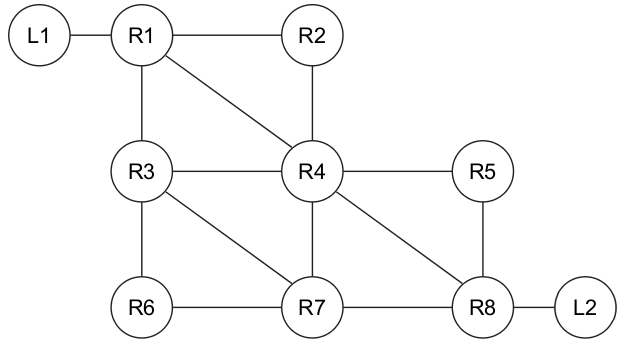
\includegraphics{data/22J2AS1_ex2.png}\{: .center width=640\}

\begin{verbatim}
=== "Réseau de transport"

    ![](data/carte-metro-parisien-768x890.jpg){: .center width=640} 

=== "Réseau social"
    ![](data/graphe_RS.png){: .center width=640} 

=== "Mais aussi"
    On trouve également des applications de la théorie des graphes dans bien d'autres domaines: ...
\end{verbatim}

!!! jeretiens ``Ce qu'il faut retenir'' D'un point de vue mathématique,
un graphe est la donnée

\begin{verbatim}
- d’un certain nombre de points du plan, appelés **_sommets_** ,  
- certains étant reliés par des segments de droites ou de courbes     (simples) appelés **_arêtes_** ,  
- la disposition des sommets et la forme choisie pour les arêtes n’intervenant pas.  
- Le nombre de sommets du graphe est son **_ordre_**.  
\end{verbatim}

\hypertarget{graphe-non-orientuxe9}{%
\subsubsection{Graphe non orienté}\label{graphe-non-orientuxe9}}

Sauf indication contraire, un graphe sera considéré comme non orienté et
les arêtes pourront être parcourues dans les deux sens.

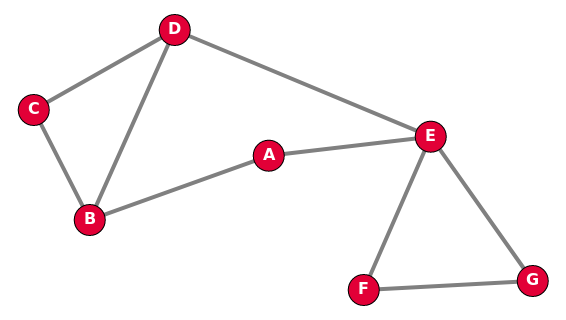
\includegraphics{data/exemple_graphe.png}\{:.center width=480\}

!!! jeretiens ``Ce qu'il faut retenir'' Dans le cas des graphes non
orientés, les relations entre deux sommets se font dans les deux sens.
On appelle ses relations des arêtes (edges en anglais), et on a les
définitions suivantes :

\begin{verbatim}
- **_Sommets adjacents_** : deux sommets sont adjacents s’ils sont reliés entre eux par une arête.  
On dit que l’arête est incidente aux deux sommets.  
- **_Voisins d’un sommet x_** : ce sont tous les sommets reliés à x par une arête.  
- **_Degré d’un sommet x_** : nombre d’arêtes incidentes au sommet, on le note d (x).  
- **_Chaîne_** : séquence ordonnée d’arêtes telle que chaque arête a une extrémité en commun avec l’arête suivante.  
- **_Cycle_** : dans un graphe non orienté, un cycle est une suite d’arêtes consécutives (chaîne) dont les deux sommets extrémités sont identiques.  
- **_Boucle_** : il peut exister des arêtes entre un sommet x et lui-même. Elles sont appelés boucles.  
\end{verbatim}

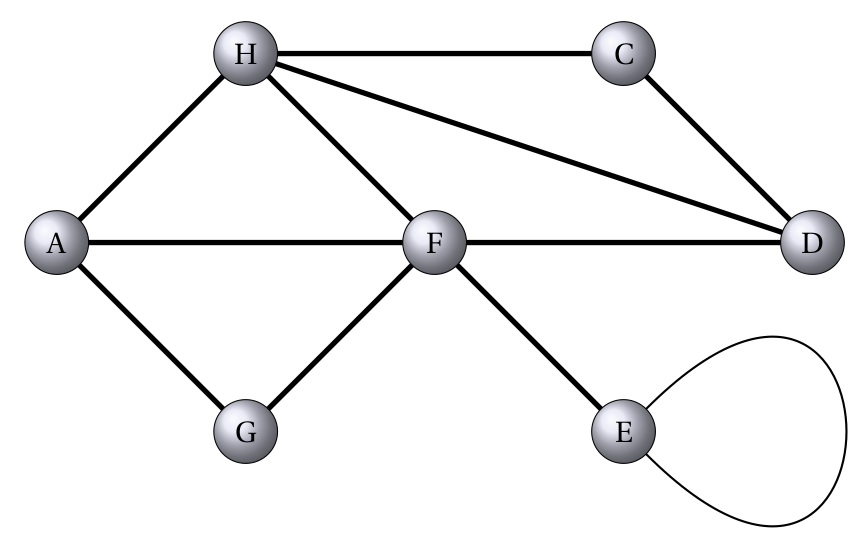
\includegraphics{data/graphe11.png}\{:.center width=450px\}

!!! exo ``Exercice 1'' - Citer des sommets adjacents.\\
- Donner le degré de chacun des sommets.\\
- Citer une chaîne.\\
- Donner un cycle.\\
- Y-t-il une boucle ?

\hypertarget{graphe-orientuxe9}{%
\subsubsection{Graphe orienté}\label{graphe-orientuxe9}}

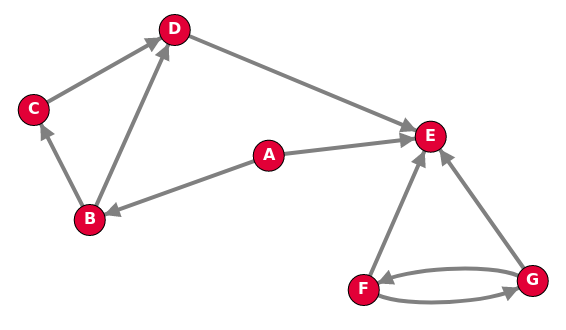
\includegraphics{data/exemple_graphe_oriente.png}\{: .center width=480\}

\begin{itemize}
\item
  Dans un graphe \textbf{orienté}, les \emph{arcs} ne peuvent être
  empruntés que dans le sens de la flèche, et un \emph{chemin} est une
  suite de sommets reliés par des arcs, comme B → C → D → E par exemple.
\item
  Les sommets C et D sont \emph{adjacents} au sommet B (mais pas A !),
  ce sont les \emph{voisins} de B.
\end{itemize}

!!! jeretiens ``Ce qu'il faut retenir'' Dans le cas des graphes
orientés, les arêtes ont un sens et elles sont appelées arcs. Par
exemple,\\
l'arête a = (x, y) indique qu'il y a un arc d'origine x et d'extrémité
finale y. De plus, on a les définitions suivantes.

\begin{verbatim}
- **_Successeurs et prédécesseurs d’un sommet x_** : dans un graphe orienté on ne parle plus de voisins d’un sommet mais de ses successeurs et de ses prédécesseurs : le successeurs de x sont tous les sommets y tels qu’il existe un arc (x, y) (de x vers y) et les prédécesseurs de x sont tous les sommets w tels qu’il existe un arc (w, x) (de w vers x).  
-  **_Chemin_** : séquence ordonnée d’arcs consécutifs (on parlait de chaîne dans un graphe non orienté).  
- **_Circuit_** : dans un graphe orienté, un circuit est une suite d’arcs consécutifs (chemin) dont les deux sommets extrémités sont identiques.  
- **_Degré d’un sommet x_** : cette notion existe aussi dans le cas des graphes orientés. On distingue le degré entrant d’un sommet x (noté $d_-(x)$= nombre de prédécesseurs de x) et le degré sortant d’un sommet x (noté $d_+(x)$= nombre de successeurs de x ). Le degré d’un sommet x vaut $d (x) = d_+(x) + d_-(x)$.  
• **_Boucle_** : ce sont les arcs entre un sommet et lui-même.
\end{verbatim}

\hypertarget{graphe-ponduxe9ruxe9}{%
\subsubsection{Graphe pondéré}\label{graphe-ponduxe9ruxe9}}

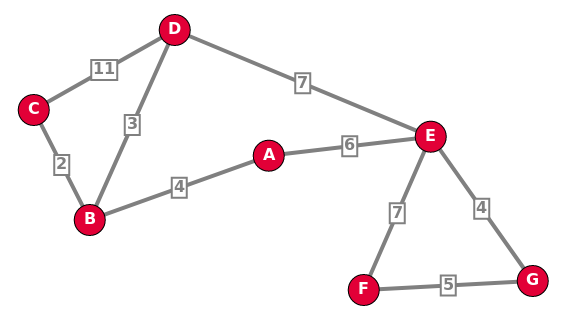
\includegraphics{data/exemple_graphe_pondere.png}\{: .center width=480\}

\begin{itemize}
\tightlist
\item
  Un graphe est \textbf{pondéré} (ou valué) si on attribue à chaque
  arête une valeur numérique (la plupart du temps positive), qu'on
  appelle \emph{mesure}, \emph{poids}, \emph{coût} ou \emph{valuation}.
\end{itemize}

Par exemple:

\begin{itemize}
\tightlist
\item
  dans le protocole OSPF, on pondère les liaisons entre routeurs par le
  coût;\\
\item
  dans un réseau routier entre plusieurs villes, on pondère par les
  distances.
\end{itemize}

\hypertarget{ruxe9seaux-sociaux-moduxe9lisation-par-un-graphe}{%
\subsection{Réseaux sociaux : modélisation par un
graphe}\label{ruxe9seaux-sociaux-moduxe9lisation-par-un-graphe}}

Au premier trimestre 2020, Facebook© revendiquait 2,6 milliards
d'utilisateurs actifs chaque mois, en hausse de 9,2\% par rapport à
début 2019. Le réseau social américain a passé la barre symbolique des 2
milliards au deuxième trimestre 2017. A noter que 42\% des utilisateurs
actifs mensuels de Facebook viennent d'Asie-Pacifique, 15,6\% sont
Européens et 9,7\% sont Nord-américains. Facebook permet à ses
utilisateurs d'entrer des informations personnelles et d'interagir avec
d'autres utilisateurs. Les interactions entre utilisateurs reposent sur
la notion « d'amis ».

\hypertarget{principe-de-la-moduxe9lisation-par-un-graphe-non-orientuxe9}{%
\subsubsection{Principe de la modélisation par un graphe non
orienté}\label{principe-de-la-moduxe9lisation-par-un-graphe-non-orientuxe9}}

Imaginez un réseau social ayant 7 abonnés (L, M, N, O, P, Q et R) où :

\begin{itemize}
\item
  L est ami avec M, N, O et P ;
\item
  M est ami avec L et P ;
\item
  N est ami avec L, O et P ;
\item
  O est ami avec L,N,P,Q et R ;
\item
  P est ami avec O,L et M ;
\item
  Q est ami avec N et O ;
\item
  R est ami avec O.
\end{itemize}

La description de ce réseau social, malgré son faible nombre d'abonnés,
est déjà quelque peu compliquée, alors imaginez cette même description
avec un réseau social comportant des millions d'entre eux !\\
Il existe un moyen plus ``visuel'' pour représenter ce réseau social :\\
on peut représenter chaque abonné par un cercle (avec le nom de l'abonné
situé dans le cercle) et chaque relation ``X est ami avec Y'' par un
segment de droite reliant X et Y (``X est ami avec Y'' et ``Y est ami
avec X'' étant représenté par le même segment de droite). Le mini-réseau
social décrit précédemment peut être modélisé sous la forme du graphe
ci-dessous :

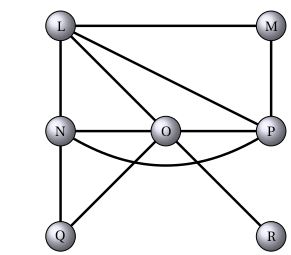
\includegraphics{data/graphe14.png}

\hypertarget{impluxe9mentation---matrice-dadjacence}{%
\subsection{Implémentation - Matrice
d'adjacence}\label{impluxe9mentation---matrice-dadjacence}}

\{\{ titre\_activite(``Implémentation avec matrice
d'adjacence'',{[}{]},0) \}\}

\begin{enumerate}
\def\labelenumi{\arabic{enumi}.}
\item
  Principe de l'implémentation\\
  On prend l'exemple du graphe orienté suivant :

  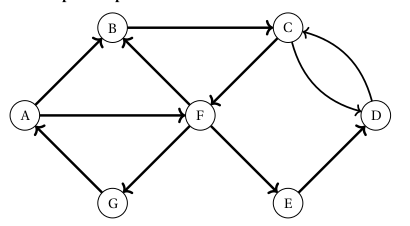
\includegraphics{data/graphe21.png}\{:.center\}

  \begin{enumerate}
  \def\labelenumii{\alph{enumii}.}
  \tightlist
  \item
    Recopier et compléter le tableau suivant dans lequel les lignes et
    les colonnes représentent les sommets et dans lequel on indique par
    un \textbf{1} la présence d'une arête allant du sommet de la ligne
    vers celui de la colonne et par \textbf{0} son absence
  \end{enumerate}

  \begin{longtable}[]{@{}ccccccc@{}}
  \toprule\noalign{}
  & A & B & C & D & E & F \\
  \midrule\noalign{}
  \endhead
  \bottomrule\noalign{}
  \endlastfoot
  A & 0 & 1 & 0 & 0 & 0 & 1 \\
  B & & & & & & \\
  C & & & & & & \\
  D & & & & & & \\
  E & & & & & & \\
  F & & & & & & \\
  \end{longtable}

  !!! note Si on numérote les sommets du graphe (A le numéro 1, B le
  numéro 2, \ldots), il n'est plus nécessaire d'indiquer les noms des
  sommets sur les lignes et les colonnes.

  \begin{enumerate}
  \def\labelenumii{\alph{enumii}.}
  \setcounter{enumii}{1}
  \tightlist
  \item
    De façon générale, une \textbf{matrice} en mathématiques est un
    tableau de nombres, ici, on a donc représenté notre graphe par une
    matrice appelé \textbf{matrice d'adjacence} de ce graphe :
  \end{enumerate}

  \begin{pmatrix}
   0 & 1 & 0 & 0 & 0 & 1 \\
   \dots & \dots  & \dots & \dots & \dots & \dots \\
   \dots & \dots  & \dots & \dots & \dots & \dots \\
   \dots & \dots  & \dots & \dots & \dots & \dots \\
   \dots & \dots  & \dots & \dots & \dots & \dots \\
   \end{pmatrix}

  En nommant les sommets A, B, C, D et E dessiner le graphe dont la
  matrice d'adjacence est :

  \begin{pmatrix}
   0 & 1 & 1 & 1 & 0 \\
   0 & 0 & 1 & 0 & 1\\
   0 & 0 & 0 & 0 & 0\\
   1 & 1 & 1 & 0 & 0\\
   0 & 0 & 0 & 1 & 0\\
   \end{pmatrix}

  \begin{enumerate}
  \def\labelenumii{\alph{enumii}.}
  \setcounter{enumii}{2}
  \item
    Que peut-on dire d'un graphe dont la matrice d'adjacence est
    symétrique par rapport à sa diagonale principale ?
  \item
    Proposer une méthode pour représenter un graphe pondéré par une
    matrice d'adjacence.
  \end{enumerate}
\item
  \textbf{Implémentation en python}\\
  On s'inspire de ce qui a été fait pour les arbres et on utilisera la
  \{\{sc(``poo'')\}\} pour représenter un graphe par sa matrice
  d'adjacence. Enfin, on suppose qu'on implémente des graphes orientés.

  \begin{enumerate}
  \def\labelenumii{\arabic{enumii}.}
  \tightlist
  \item
    Pour le constructeur de la classe Graphe, on propose de fournir
    uniquement les sommets et de créer l'objet graphe ayant sa matrice
    d'adjacence vide initialement. De plus on ajoute un attribut
    \texttt{taille} au graphe. Compléter le code ci-dessous :
  \end{enumerate}

\begin{Shaded}
\begin{Highlighting}[]
\KeywordTok{class}\NormalTok{ Graphe:}

    \KeywordTok{def} \FunctionTok{\_\_init\_\_}\NormalTok{(}\VariableTok{self}\NormalTok{,sommets):}
        \VariableTok{self}\NormalTok{.sommets}\OperatorTok{=}\NormalTok{sommets}
        \VariableTok{self}\NormalTok{.taille }\OperatorTok{=} \BuiltInTok{len}\NormalTok{(......)}
        \VariableTok{self}\NormalTok{.matrice }\OperatorTok{=}\NormalTok{ .............  }\CommentTok{\#construction par compréhension avec que des 0}
\end{Highlighting}
\end{Shaded}

  \begin{enumerate}
  \def\labelenumii{\arabic{enumii}.}
  \setcounter{enumii}{1}
  \item
    Poursuivre cette implémentation en ajoutant une méthode d'ajout
    d'une arête.

    !!! aide * Cette méthode prend en paramètre l'origine et l'extrémité
    de l'arête à ajouter. * On pourra vérifier que l'origine et
    l'extrémité sont bien dans la liste de sommets et rechercher leur
    position grâce à la méthode \texttt{index} des listes de python.
  \item
    Ajouter une méthode de suppression d'une arête
  \item
    Ajouter une méthode d'affichage de la matrice d'adjacence
  \item
    Ecrire la méthode \texttt{voisins} qui prend en paramètre un sommet
    et renvoie la liste de ses voisins.
  \end{enumerate}
\end{enumerate}

\{\{ titre\_activite(``Implémentation avec des listes
d'adjacences'',{[}{]}) \}\}

\begin{enumerate}
\def\labelenumi{\arabic{enumi}.}
\item
  \textbf{Principe de l'implémentation}\\
  On reprend l'exemple du graphe orienté déjà utilisé à l'activité
  précédente

  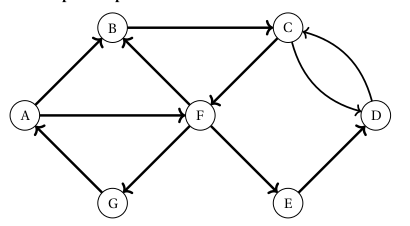
\includegraphics{data/graphe21.png}\{:.center\}

  \begin{enumerate}
  \def\labelenumii{\alph{enumii}.}
  \tightlist
  \item
    Compléter le schéma suivant où on a fait figuré à côté de chaque
    sommet la liste des sommets adjacents :
  \end{enumerate}

  \begin{itemize}
  \tightlist
  \item
    \texttt{A\ :\ B,F}
  \item
    \texttt{B\ :\ ...}
  \item
    \texttt{C\ :\ ...}
  \item
    \texttt{.\ :\ ...}
  \item
    \texttt{.\ :\ ...}
  \item
    \texttt{.\ :\ ...}
  \end{itemize}

  \begin{enumerate}
  \def\labelenumii{\alph{enumii}.}
  \setcounter{enumii}{1}
  \tightlist
  \item
    Dessiner le graphe dont la représentation par liste d'adjacence est
    :
  \end{enumerate}

  \begin{itemize}
  \tightlist
  \item
    \texttt{R\ :\ S}
  \item
    \texttt{S\ :\ R,T,U,V}
  \item
    \texttt{T\ :\ V}
  \item
    \texttt{U\ :\ None}
  \item
    \texttt{V\ :\ R,U}
  \end{itemize}
\item
  Implémentation en Python\\
  On donne ci-dessous le constructeur d'une classe \texttt{Graphe} qui
  implémente les graphes sous la forme de listes d'adjacence :

\begin{Shaded}
\begin{Highlighting}[]
\KeywordTok{class}\NormalTok{ Graphe:}

    \KeywordTok{def} \FunctionTok{\_\_init\_\_}\NormalTok{(}\VariableTok{self}\NormalTok{,sommets):}
        \VariableTok{self}\NormalTok{.taille }\OperatorTok{=} \BuiltInTok{len}\NormalTok{(sommets)}
        \VariableTok{self}\NormalTok{.listes }\OperatorTok{=}\NormalTok{ \{\}}
        \ControlFlowTok{for}\NormalTok{ s }\KeywordTok{in}\NormalTok{ sommets:}
            \VariableTok{self}\NormalTok{.listes[s]}\OperatorTok{=}\NormalTok{[]}
\end{Highlighting}
\end{Shaded}

  \begin{enumerate}
  \def\labelenumii{\alph{enumii}.}
  \item
    Quel est le type de l'attribut \texttt{listes} d'un objet de la
    classe \texttt{Graphe} ?
  \item
    On suppose qu'on crée un objet de la classe \texttt{Graphe} en
    donnant en paramètre la liste \texttt{{[}"A","B","C","D"{]}}. Quel
    est alors le contenu de l'attribut \texttt{listes} de cet objet ?
  \item
    Poursuivre cette implémentation en ajoutant une méthode d'ajout
    d'une arête.
  \item
    Ajouter une méthode de suppression d'une arête
  \item
    Proposer une méthode permettant d'ajouter un sommet.
  \item
    Proposer une méthode permettant de supprimer un sommet.
  \item
    Ecrire la méthode \texttt{voisins} qui prend en paramètre un sommet
    et renvoie la liste de ses voisins.
  \end{enumerate}
\end{enumerate}

\{\{ titre\_activite(``Parcours d'un graphe'',{[}{]}) \}\}

\begin{enumerate}
\def\labelenumi{\arabic{enumi}.}
\item
  Visualisation d'un parcours \emph{depth first search}\\
  Un
  \href{https://workshape.github.io/visual-graph-algorithms/\#dfs-visualisation}{outil
  en ligne}, permet de visualiser le résultat du parcours en profondeur
  d'un graphe. Un graphe est donné en exemple, mais vous pouvez le
  modifier ou construire le votre.
  \href{https://workshape.github.io/visual-graph-algorithms/\#dfs-visualisation}{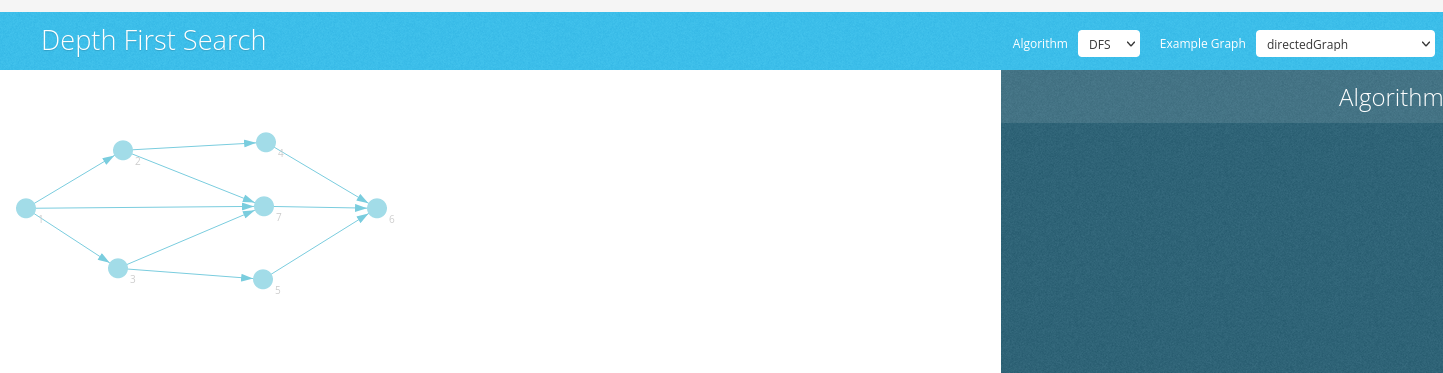
\includegraphics{data/dfs.png}\{:
  width=600px .imgcentre\}}

  !!! attention Dans les menus déroulants, bien choisir Alorithme :
  \textbf{DFS} et Example graph : \textbf{directedGraph}
\item
  Visualisation d'un parcours \emph{breadth first search}\\
  Ce même
  \href{https://workshape.github.io/visual-graph-algorithms/\#bfs-visualisation}{outil
  en ligne}, permet de visualiser le résultat du parcours en largeur
  d'un graphe. Un graphe est donné en exemple, mais vous pouvez le
  modifier ou construire le votre :
  \href{https://workshape.github.io/visual-graph-algorithms/\#bfs-visualisation}{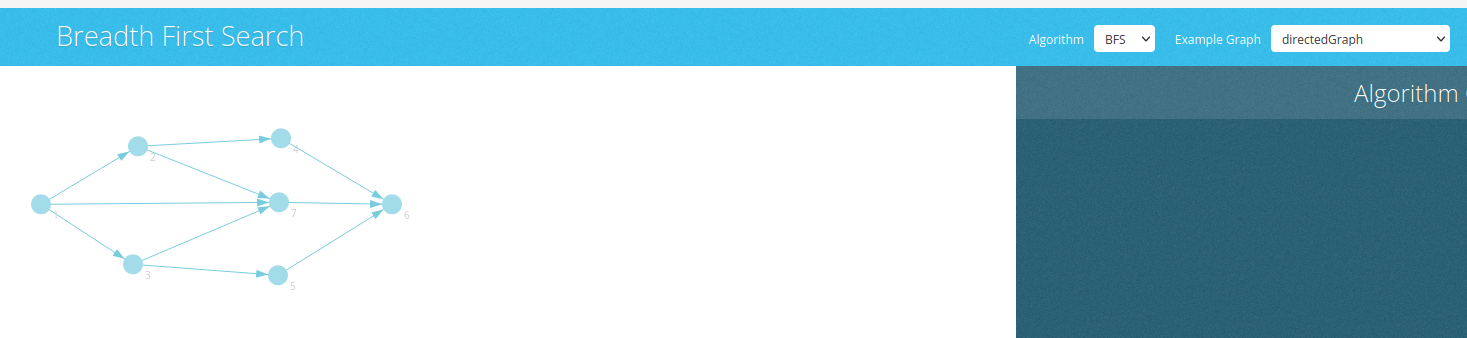
\includegraphics{data/bfs.png}\{:
  width=600px .imgcentre\}}

  !!! attention Dans les menus déroulants, bien choisir Alorithme :
  \textbf{BFS} et Example graph : \textbf{directedGraph}
\item
  On considère le graphe suivant :\\

  \texttt{mermaid\ \ \ \ \ graph\ LR\ \ \ \ \ A(("A"))\ \ \ \ \ B(("B"))\ \ \ \ \ C(("C"))\ \ \ \ \ D(("D"))\ \ \ \ \ E(("E"))\ \ \ \ \ F(("F"))\ \ \ \ \ G(("G"))\ \ \ \ \ A\ -\/-\textgreater{}\ B\ \ \ \ \ A\ -\/-\textgreater{}\ C\ \ \ \ \ B\ -\/-\textgreater{}\ D\ \ \ \ \ C\ -\/-\textgreater{}\ F\ \ \ \ \ C\ -\/-\textgreater{}\ G\ \ \ \ \ E\ -\/-\textgreater{}\ G\ \ \ \ \ A\ -\/-\textgreater{}\ E\ \ \ \ \ D\ -\/-\textgreater{}\ F\ \ \ \ \ G\ -\/-\textgreater{}\ F\ \ \ \ \ B\ -\/-\textgreater{}\ C}

  \begin{enumerate}
  \def\labelenumii{\alph{enumii}.}
  \item
    Prévoir l'ordre de parcours pour un parcours en profondeur en
    commençant par le sommet \texttt{A}. Vérifier en testant dans
    l'outil en ligne.
  \item
    Même question pour un parcours en largeur.
  \end{enumerate}
\end{enumerate}

\hypertarget{exercices}{%
\subsection{Exercices :}\label{exercices}}

\{\{ exo(``Vocabulaire sur les graphes'',{[}{]},0) \}\}

On considère le graphe suivant :

\begin{Shaded}
\begin{Highlighting}[]
\NormalTok{graph LR}
\NormalTok{A(("A"))}
\NormalTok{B(("B"))}
\NormalTok{C(("C"))}
\NormalTok{D(("D"))}
\NormalTok{E(("E"))}
\NormalTok{F(("F"))}
\NormalTok{G(("G"))}
\NormalTok{H(("H"))}
\NormalTok{A {-}{-}{-} B}
\NormalTok{A {-}{-}{-} C}
\NormalTok{C {-}{-}{-} F}
\NormalTok{C {-}{-}{-} G}
\NormalTok{E {-}{-}{-} G}
\NormalTok{G {-}{-}{-} F}
\NormalTok{B {-}{-}{-} E}
\NormalTok{C {-}{-}{-} H}
\NormalTok{B {-}{-}{-} D}
\NormalTok{D {-}{-}{-} C}
\end{Highlighting}
\end{Shaded}

\begin{verbatim}
</div>
\end{verbatim}

\begin{enumerate}
\def\labelenumi{\arabic{enumi}.}
\tightlist
\item
  Ce graphe est-il orienté ? simple ? complet ? pondéré ?\\
\item
  Donner la liste des voisins de \texttt{C}.\\
\item
  Quel est le degré de \texttt{G} ?\\
\item
  Quels sont les sommets adjacents à \texttt{A} ?
\end{enumerate}

\{\{ exo(``Graphe complet'',{[}{]}) \}\}

\begin{enumerate}
\def\labelenumi{\arabic{enumi}.}
\item
  Rappeler la définition d'un graphe \emph{complet}\\
\item
  Dessiner un graphe complet à cinq noeuds.\\
\item
  Combien d'arêtes possède ce graphe ?\\
\item
  Donner la matrice d'adjacence de ce graphe.\\
\item
  Quel est le nombre d'arêtes d'un graphe complet à \(n\) noeuds ?

  !!! aide On pourra utiliser sans avoir à le prouver que : \$ 1 + 2 +
  \dots + n = \dfrac{n(n+1)}{2} \$
\end{enumerate}

\{\{ exo(``Représentation par matrice d'adjacence'',{[}{]}) \}\}

\begin{enumerate}
\def\labelenumi{\arabic{enumi}.}
\item
  Donner la matrice d'adjacence du graphe suivant :

  \texttt{mermaid\ \ \ \ \ graph\ LR\ \ \ \ \ A(("A"))\ \ \ \ \ B(("B"))\ \ \ \ \ C(("C"))\ \ \ \ \ D(("D"))\ \ \ \ \ E(("E"))\ \ \ \ \ A\ -\/-\/-\ B\ \ \ \ \ A\ -\/-\/-\ C\ \ \ \ \ C\ -\/-\/-\ E\ \ \ \ \ D\ -\/-\/-\ E\ \ \ \ \ B\ -\/-\/-\ C\ \ \ \ \ C\ -\/-\/-\ D}
\item
  Dessiner le graphe dont la matrice d'adjacence est :

  \begin{pmatrix}
  0 & 1 & 1 & 0 & 0 \\
  0 & 0 & 1 & 0 & 1 \\
  1 & 1 & 0 & 0 & 0 \\
  0 & 1 & 1 & 0 & 0 \\
  0 & 1 & 1 & 0 & 0 \\
  \end{pmatrix}
\end{enumerate}

\{\{ exo(``Représentation par listes d'adjacence'',{[}{]}) \}\}

\begin{enumerate}
\def\labelenumi{\arabic{enumi}.}
\item
  Donner la représentation sous forme de listes d'adjacences du graphe
  suivant :

  \texttt{mermaid\ \ \ \ \ graph\ LR\ \ \ \ \ A(("A"))\ \ \ \ \ B(("B"))\ \ \ \ \ C(("C"))\ \ \ \ \ D(("D"))\ \ \ \ \ E(("E"))\ \ \ \ \ A\ -\/-\/-\ B\ \ \ \ \ A\ -\/-\/-\ C\ \ \ \ \ C\ -\/-\/-\ E\ \ \ \ \ D\ -\/-\/-\ E\ \ \ \ \ B\ -\/-\/-\ C\ \ \ \ \ C\ -\/-\/-\ D}
\item
  Dessiner le graphe dont la représentation sous forme de listes
  d'adjacence est :

  \begin{itemize}
  \tightlist
  \item
    A : {[}B{]}
  \item
    B : {[}C,D,E{]}
  \item
    C : {[}F{]}
  \item
    D : {[}F{]}
  \item
    E : {[}F{]}
  \end{itemize}
\end{enumerate}

\{\{ exo(``Parcours d'un graphe'',{[}{]}) \}\}

On considère le graphe suivant :

\begin{verbatim}
```mermaid
graph LR
A(("A"))
B(("B"))
C(("C"))
D(("D"))
E(("E"))
F(("F"))
G(("G"))
A --> B
A --> C
G --> E
C --> D
D --> F
B --> E
E --> F
A --> G
```
</div>
\end{verbatim}

\begin{enumerate}
\def\labelenumi{\arabic{enumi}.}
\tightlist
\item
  Donner l'ordre de parcours des sommets pour un parcours en largeur en
  partant de A
\item
  Même question pour un parcours en profondeur
\end{enumerate}

\{\{ exo(``Implémentation par matrice d'adjacence'',{[}{]}) \}\}

\begin{enumerate}
\def\labelenumi{\arabic{enumi}.}
\item
  Récupérer, et revoir l'implémentation des graphes réalisée précédement
  :\\
  \{\{ telecharger(``Implémentation graphes par
  matrice'',``../files/C22/graphes\_matrice.py'')\}\}
\item
  Utiliser cette implémentation pour créer le graphe de sommets
  \texttt{A,B,C,D,E} et dont la matrice d'adjacence est :

  \begin{pmatrix}
  0 & 1 & 1 & 0 & 0 \\
  0 & 0 & 1 & 0 & 0 \\
  0 & 0 & 0 & 1 & 1 \\
  0 & 0 & 0 & 0 & 0 \\
  0 & 0 & 0 & 0 & 0 \\
  \end{pmatrix}
\item
  Ajouter la méthode \texttt{parcours\_largeur} ci-dessous à cette
  implémentation en la complétant.
\end{enumerate}

\begin{Shaded}
\begin{Highlighting}[]
\KeywordTok{def}\NormalTok{ parcours\_largeur(}\VariableTok{self}\NormalTok{,depart):}
        \ControlFlowTok{assert}\NormalTok{ depart }\KeywordTok{in} \VariableTok{self}\NormalTok{.sommets}
\NormalTok{        a\_traiter }\OperatorTok{=}\NormalTok{ [depart]}
\NormalTok{        deja\_vu }\OperatorTok{=}\NormalTok{ [depart]}
\NormalTok{        pl  }\OperatorTok{=}\NormalTok{ []}
        \ControlFlowTok{while}\NormalTok{ a\_traiter }\OperatorTok{!=}\NormalTok{ []:}
\NormalTok{            sommet }\OperatorTok{=}\NormalTok{ a\_traiter[}\DecValTok{0}\NormalTok{]}
\NormalTok{            voisins }\OperatorTok{=} \VariableTok{self}\NormalTok{.get\_voisin(sommet)}
            \CommentTok{\# Ajout des sommets voisins non encore parcourus à ceux à traiter}
            \ControlFlowTok{for}\NormalTok{ v }\KeywordTok{in}\NormalTok{ .......:}
                \ControlFlowTok{if}\NormalTok{ v }\KeywordTok{not} \KeywordTok{in}\NormalTok{ .....:}
\NormalTok{                    a\_traiter......(v)}
\NormalTok{                    deja\_vu.......(v)}
\NormalTok{            pl.append(sommet)}
\NormalTok{            a\_traiter.....(}\DecValTok{0}\NormalTok{)}
        \ControlFlowTok{return}\NormalTok{ pl}
\end{Highlighting}
\end{Shaded}

\begin{enumerate}
\def\labelenumi{\arabic{enumi}.}
\setcounter{enumi}{3}
\item
  Reconnaître la structure de données utilisée pour la variable
  \texttt{a\_traiter}, expliquer pourquoi le choix d'une liste n'est pas
  judicieux.
\item
  Ajouter la méthode \texttt{parcours\_profondeur} ci-dessous à cette
  implémentation en la complétant.
\end{enumerate}

\begin{Shaded}
\begin{Highlighting}[]
\KeywordTok{def}\NormalTok{ parcours\_profondeur(}\VariableTok{self}\NormalTok{,start,parcourus}\OperatorTok{=}\VariableTok{None}\NormalTok{):}
        \ControlFlowTok{if}\NormalTok{ parcourus }\OperatorTok{==} \VariableTok{None}\NormalTok{:}
\NormalTok{            parcourus }\OperatorTok{=}\NormalTok{ []}
\NormalTok{        parcourus.append(start)}
        \ControlFlowTok{for}\NormalTok{ v }\KeywordTok{in} \VariableTok{self}\NormalTok{...........(start):}
            \ControlFlowTok{if}\NormalTok{ v }\KeywordTok{not} \KeywordTok{in}\NormalTok{ parcourus:}
                \VariableTok{self}\NormalTok{............(v,parcourus)}
        \ControlFlowTok{return}\NormalTok{ parcourus}
\end{Highlighting}
\end{Shaded}

\begin{enumerate}
\def\labelenumi{\arabic{enumi}.}
\setcounter{enumi}{5}
\item
  Proposer une méthode permettant d'ajouter un sommet.
\item
  Proposer une méthode permettant de supprimer un sommet.
\end{enumerate}

\{\{ exo(``Implémentation par listes d'adjacence'',{[}{]}) \}\}

Reprendre les questions de l'exercice précédent avec l'implémentation
par liste d'adjacence :\\
\{\{ telecharger(``Implémentation graphes par
listes'',``../files/C22/graphes\_liste.py'')\}\}



\end{document}
